\chapter{Punktesortierung in Schachbrettmustern}
\label{sec:schachbrettAlg} 


Für die Detektion von korrespondierenden Punkten in Stereoskopischen Bildaufnahmen von zweidimensionalen Schachbrettern, ist ein Algorithmus entwickelt worden, welcher die zuvor Detektierten Eckpunkte eines Schachbretts sortiert und eindeutig identifiziert. Jeder Punkt beinhaltet nach der Sortierung die Information in welcher Reihe $j$ und in welcher Spalte $i$ er sich befindet. Jeder Punkt ist somit eindeutig durch die zwei Indizes $i$ und $j$ identifiziert. Dem entstandenen Sorierungsalgorithmus ist ein Algorithmus zu Detektion der Eckpunkte eines Schacbretts voran geschaltet. Werden beide Algorithmen auf die Stereoaufnahme zweier Schachbretter angewandt, so können korrespondierende Punkte anhand dieser Indizes ausgemacht werden. Die Schachbretter können dabei sowohl Kissen- als auch Tonnennverzeichnungen aufweisen und oder perspektivisch verzerrt sein.\\ 



%Das Bild des Schachbretts wird in ein zweidimensionales Koordinatensystem $(A,\alpha)$ mit $\alpha = (j,i)$ gelegt. 

%Als erstes wird ein Startpunkt innerhalb des Schachbretts gesucht. 

Aus den zuvor detektierten Eckpunkten des Schachbretts wird ein Startpunkt gesucht. Der Startpunkt wird so bestimmt, dass es immer die linke unterste Ecke des Schachbretts ist. Somit ist gewährleistet, dass die Indizes der Eckpunkte beider Bilder gleich sind. Ist der Startpunkt bestimmt, bekommt dieser die Indizes $i = 1$ und $j = 1$. $i$ steht für die jeweilige Reihen in welcher sich ein Punkt befindet und $j$ steht für die jeweilige Spalte. Ist der Startpunkt bestimmt, wird der erste Punkt entlang der unteren Schachbrettkante in $j$-Richtung und der erste Punkt entlang der linken Randkante in $i$-Richtung gesucht. Anhand dieser Punkte lassen sich vom Startpunkt aus Richtungsvektoren definieren. Mit Hilfe des Richtungsvektors, wird ein Suchbereich definiert, mit dessen Hilfe der nächste Punkt entlang der jeweiligen $i$-und $j$-Richtung 



Anhand der ersten Punkte, können vom Startpunkt aus zwei Richtungsvektoren bestimmt werden. Die Richtungsvektoren ...\\



(WEITER SCHREIBEN!!!!!)\\


\begin{figure}[!htb]
	\centering
	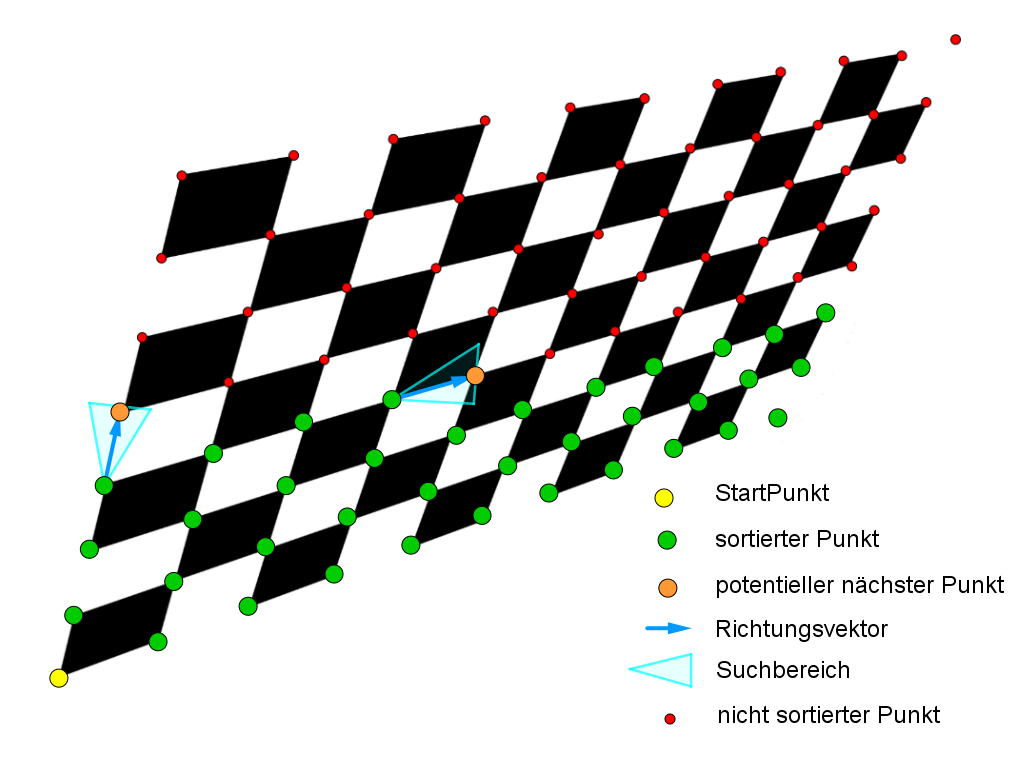
\includegraphics[width=0.8\linewidth]{images/VerzeichnetesSchachbretFunktion.png}
	\caption[Funktionsübersicht des Sorieralgorithmus]{In der Abbildung ist die Vorgehensweise des Sortierungsalgorithmus schematisch zu sehen.}
	\label{fig:UebersichtSortierungsAlg}
\end{figure}




\section{Sortierungsalgorithmus}

Für die Sortierung der Schachbrettpunkte, wird das Schachbrett in ein Koordinatensystem, mit vertikaler Achse $i$ und horizontaler Achse $j$, gelegt. Um das Schachbrett herum wird ein Rahmen definiert. Die Punkte mit der maximale $i$-Koordinate und der minimalen $i$-Koordinate Begrenzen die oberen und unteren Kanten des Rahmens. Die Punkte mit der minimalen $j$-Koordinate und der Punkt mit der  maximalen $j$-Koordinate Begrenzen die vertikalen Kanten des Rahmens. In Abbildung \ref{fig:7.1} sind die roten Begrenzungskanten um das Schachbrett zu sehen.\\

Der durch den Rahmen begrenzte Bereich wird in gleich viele Reihen wie Spalten unterteilt, so dass eine Gitter entsteht. Die so entstehenden Zellen des Gitters werden in $i$-Richtung sowie in $j$-Richtung durchgezählt und bekommen somit jeweils zwei Indizes $(i_i,j_i)$, welche sie eindeutig identifizieren.\\

In den angelegten $ConstantArrays$ namens $JSplits$ und $ISplits$ werden die Begrenzungen Zellen in $i$- und $j$-Richtung gespeichert. Die Begrenzungen der Zellen werden über die Distanz des Punktes mit der minimalen $j$-Koordinate zum Punkt mit der maximalen $j$-Koordinate geteilt durch die gewünschte Anzahl der Zellen, definiert. Selbiges gilt für die Unterteilung der Zellen in $i$-Richtung. \\ 

Alle Punkte in den Zellen mit den Indizes $i=1$ und $j \leq  j_{max}$ werden als mögliche Startpunkte gekennzeichnet. In Abbildung \ref{fig:7.1} befinden sich die möglichen Startpunkte innerhalb des blauen Bereichs. Die Suche nach einem Startpunkt und auch nach den ersten Punkten in zwei Richtungen vom Startpunkt aus, ist relativ komplex. Der Grund hierfür ist, dass sämtliche Schachbretter wie in \ref{sec:SchachAlgBeispiele} gezeigt, in Betracht gezogen werden müssen. Um Anhand des Algorithmus später korrespondierende Punkte in zwei Aufnahmen des Schachbretts finden kann, sollte gewährleistet sein, dass der Startpunkt immer an der selben Ecke eines Schachbretts platziert wird.\\

\begin{figure}[!htb]
	\centering
	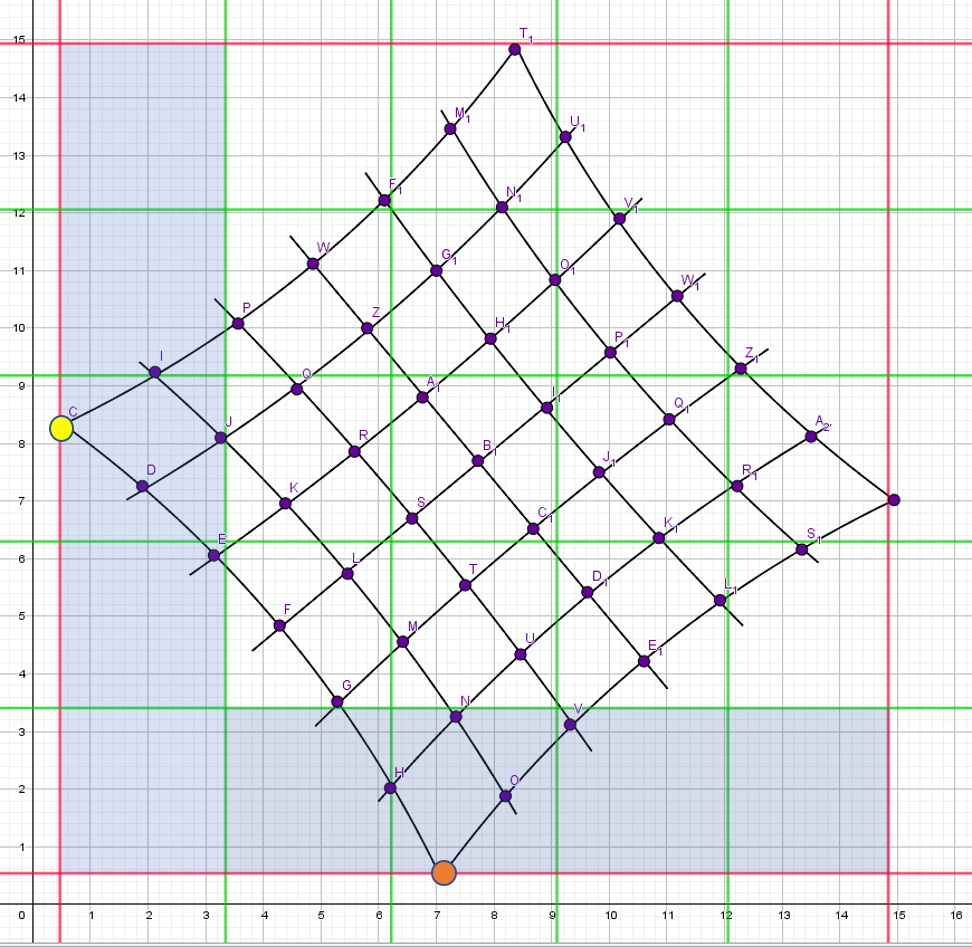
\includegraphics[width=0.6\linewidth]{images/VerzeichnetesSchachbrett_1.png}
	\caption[Startpunktsuche in Schachbrettpunkten]{Die in blau markierten Bereiche beinhalten die möglichen Startpunkte. Der Bereich entlang der horizontalen $j$- Achse bildet die erste Suchfensterreihe in $i$-Richtung. Der blaue Bereich entlang der vertikalen $i$-Achse bildet die erste Suchfensterreihe in $j$-Richtung. Der gelbe Punkt steht für den Punkt welcher als $VecJ$ bezeichnet wurde und der orange Punkt ist derjenige Punkt, welcher als $VecI$ bestimmt wurde}
	\label{fig:7.1}
\end{figure}

Innerhalb der blau gefärbten Fläche, wie sie in Abbildung \ref{fig:7.1} abgebildet ist, wird nach einem Startpunkt gesucht. Die Suche nach einem Startpunkt wird pro $i$- und $j$-Richtung in zwei Abfragen unterteilt.\\


In der ersten Abfrage für die $i$-Richtung, wird innerhalb der ersten Zellenreihe entlang der $j$- Koordinatenachse nach dem Punkt mit der kleinsten $i$-Koordinate gesucht.Dieser Punkt wird als möglicher erster Startpunkte in der Variablen $VecI$ gespeichert.\\


Danach wird geprüft ob es innerhalb der ersten Zellen in $i$-Richtung einen weiteren Punkt gibt dessen $j$-Koordinate kleiner ist als die des momentan gesetzten Punktes $VecI$, wird ein solcher Punkt gefunden, so wird dieser Punkt als neuer $VecI$ gesetzt, sofern seine $i$-Koordinate nicht größer ist als die des zuvorigen $VecI$ plus einem Pufferwert. Durch den Puffer wird verhindert, dass ein Punkt als $VecI$ gesetzt wird, welcher sich möglicherweise schon in der zweiten Reihe der Schachbrettpunkte befinden würde. In Abbildung \ref{fig:7.1} ist $VecI$ mit als oranger Punkt abgebildet.\\

%\begin{figure}[!htb]
%	\minipage{0.48\textwidth}
%	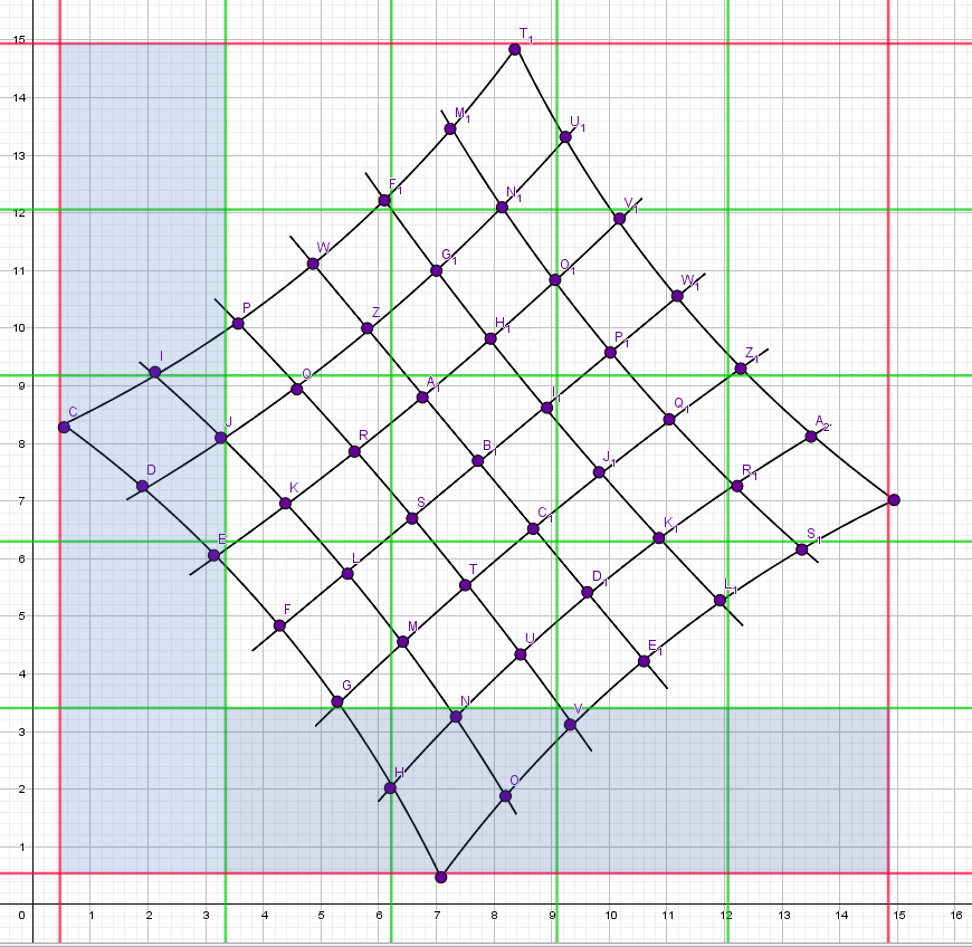
\includegraphics[width=\linewidth]{images/VerzeichnetesSchachbrett_0.png}
%	\caption{ }
%	\label{fig:7.1}
%\end{figure}
%	\endminipage\hfill


Für die erste Abfrage in $j$-Richtung, werden die Zellen entlang der vertikalen $i$-Koordinatenachse mit den Indizes $j=1$ und $i \leq i_{max}$, nach dem Punkt gesucht, welcher die geringste $j$-Koordinate besitzt. Dieser Punkt wird als vorläufiges $VecJ$ bestimmt.\\

Danach wird auch hier geprüft, ob es innerhalb der ersten Suchfensterreihe in $j$-Richtung einen weiteren Punkt gibt, dessen $i$-Koordinate kleiner ist als die des momentan gesetzten Punktes $VecJ$. Trifft des Weiteren zu, dass die $j$-Koordinaten des neu gefundenen Punktes kleiner ist als die $j$-Koordinate plus einem Pufferwert des momentanen $VecJ$ , so wird dieser als neuer Punkt als $VecJ$ festgelegt. In Abbildung \ref{fig:7.1} ist $VecJ$ als gelber Punkt zu sehen.\\

Je nachdem wie das Schachbrett liegt oder welche Verzerrungen es aufweist, kann es sein dass $VecI$ und $VecJ$ den selben Punkt ergeben haben, was den Startpunkt $StartPoint$ eindeutig identifiziert, wie es in Beispiel \ref{fig:Extreme1} oder auch \ref{fig:Extreme5} der Fall ist. Andererseits kann es auch wie in Abbildung \ref{fig:7.1} zu sehen ist, sein, dass $VecI$ und $VecJ$ sich unterscheiden. In solchen Fällen wird $VecJ$ als Startpunkt festgelegt wird. Somit ist gewährleistet, das je nach Lage des Schachbretts der linke obere oder die linke untere Ecke des Schachbretts als Startpunkt gesetzt werden\\

Die Koordinaten des $Startpoint$ werden in eine Liste aus $Associations$ \cite{Mathematica} hinzugefügt. $Associations$ können Werten Schlüsselwörter zuweisen. Anhand dieser Schlüssel sind Werte eindeutig identifiziert. 

Die $Association$-Liste $SortedPoints$ beinhaltet die Schlüssel $CoordJ$ und $CoordI$, welche die jeweiligen $i$- und $j$- Koordinaten des Punktes speichern. Die Schlüssel $CellI$ und $CellJ$, speichern die Information in welcher Zelle sich der Startpunkt befindet und die Schlüssel $NeighbourI$ und $NeighbourJ$ speichern die Indizes $i$ und $j$ ab, die definieren, der wievielte Punkt $StartPoint$ in $i$-Richtung und in $j$-Richtung ist. Er bekommt als erster Sortierter Punkte die $NeighbourI = 1$ und $NeighbourJ = 1$ zugeordnet. Ein Eintrag für einen Punkt in der Liste $SortedPoints$ sieht wie folgt aus \\

\begin{gather*}
	\begin{split}
			StartPoint &= \{ <|CoordI \rightarrow i-\text{Koordinate},\, CoordJ \rightarrow j-\text{Koordinat},\, \\
			&CellI \rightarrow i-\text{Zelle},\, CellJ \rightarrow j-\text{Zelle},\,
			NeighbourI \rightarrow 1, \,NeighbourJ \rightarrow 1  |>\}
	\end{split}
\end{gather*}
 
Anhand der Schlüssel $NeighbourI$ und $NeighbourJ$, können Punkte eindeutig identfiziert werden, da die in den Schlüssel die Information steckt, in welcher Reihe von $i$ und in welcher Spalte von $j$ sich ein Punkt aufhält und welche Punkte sind mit ihm in der selben Reihe oder Spalte. In den Abbildungen \ref{fig:Extreme1} bis \ref{fig:Extreme10} wurden die Punkte angefragt welche sich in der dritten Reihe von $i$ befinden. Besagte Punkte sind in den Grafiken grün eingefärbt.\\

Die Schlüssel $ICoord$ und $JCoord$ werden noch in eine weitere Liste namens $CheckList$ gespeichert. Anhand der $CheckList$ wird überprüft, ob die Koordinatend und somit ein Punkt selbst bereits Sortiert wurde. Damit wird verhindert, dass ein Punkt mehrmals in einsortiert wird.\\
 
Nachdem der Startpunkt gefunden ist werden die nächsten Punkte in $i$- und $j$-Richtung gesucht. Diese Punkte werden später in die Variablen $NextI$ und $NextJ$ gespeichert. In Abbildung \ref{fig:NextINextJ} ist $NextI$ der violette Punkte und $NextJ$ ist der rote Punkte. \\

Für die Bestimmung von $NextI$ wird zu erst initial $NextI = <|CoordI \rightarrow 100 000, CoordJ \rightarrow 100 000|>$ gesetzt. Es werden Punkte gesucht, welche sich in der selben $CellI$ wie $StartPoint$ und in den Zellen eins darüber $CellI +1$ und eine darunter $CellI-1$ befinden. In Abbildung \ref{fig:NextINextJ} ist der Bereich gelb eingefärbt.\\


\begin{figure}[!htb]
	\centering
	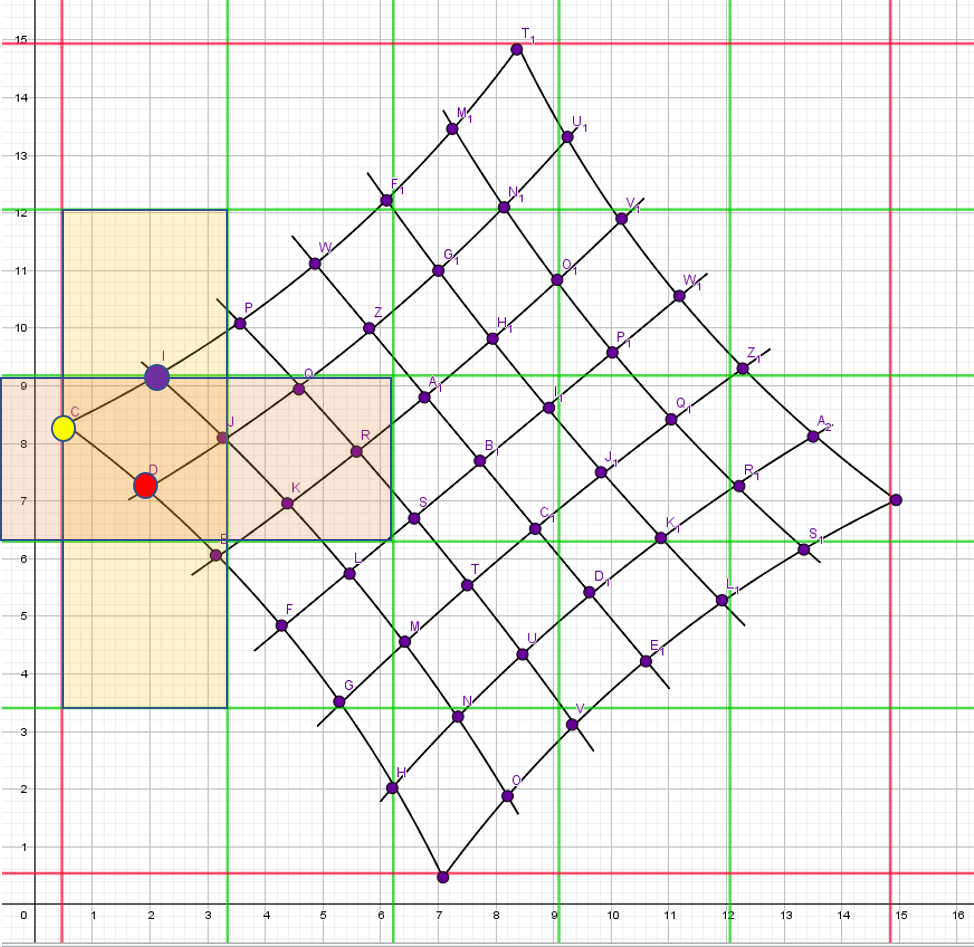
\includegraphics[width=0.6\linewidth]{images/VerzeichnetesSchachbrett_2.png}
	\caption[Finden der Startvektoren in Schachbrettpunkten]{Der in gelb markierte Bereich beinhaltet die für $NextI$ möglichen Punkte. der orange markierte Bereich beinhaltet die für $NextJ$ möglichen Punkte. Der violett gefärbe Punkt ist der gesuchte $NextI$, der rot gefärbte Punkt ist der gesuchte $NextJ$}
	\label{fig:NextINextJ}
\end{figure}


Gibt es in diesem Bereich einen Punkt, dessen $i$-Koordinate größer ist als die $i$-Koordinate des $StartPoints$ und dessen $j$-Koordinate kleiner ist als die des momentan gesetzten $NextI$, so wird dieser Punkt als neues $NextI$ festgelegt. Danach wird geprüft, ob der neue $NextI$ schon der letztendliche $NextI$ ist. Um das zu prüfen wird zunächst überprüft ob es innerhalb des gelben Bereichs noch einen Punkt gibt, dessen $j$-Koordinatenabstand vom Startpunkt aus kleiner gleich dem $j$-Koordinatenabstand zwischen dem momentanen $NextI$ zum Startpunkt ist. Gleichzeitig wird auch noch geprüft, ob der $i$-Koordinatenabstand zwischen $StartPoint$ und $NextI$ größer ist als der $i$-Koordinatenabstand zwischen einem Punkt innerhalb des Bereichs und $StartPoint$. Ist dies der Fall, so wird der gefundenen Punkt als neues $NextI$ bestimmt. Für die Überprüfung mit $NextJ$ wird nach dem gleichen Schema verfahren. in Abbildung \ref{fig:FindNextIJ} ist die eben beschriebene Prüfung nochmal grafisch dargestellt. $NextI$ und $NextJ$ werden dann mit den selben Schlüssel aber anderen zugeteilten Werten wie $StartPoint$ in die Liste $SortedPoints$ geschrieben. Die $CheckList$ wird um die Punkte $NextI$ und $NextJ$ erweitert.


\begin{gather*}
	\begin{split}
		NextI &= \{ <|CoordI \rightarrow i-\text{Koordinate},\, CoordJ \rightarrow j-\text{Koordinat},\, \\
		&CellI \rightarrow i-\text{Zelle},\, CellJ \rightarrow j-\text{Zelle},\,
		NeighbourI \rightarrow 2, \,NeighbourJ \rightarrow 1  |>\}
	\end{split}\\
	\begin{split}
	NextJ &= \{ <|CoordI \rightarrow i-\text{Koordinate},\, CoordJ \rightarrow j-\text{Koordinat},\, \\
	&CellI \rightarrow i-\text{Zelle},\, CellJ \rightarrow j-\text{Zelle},\,
	NeighbourI \rightarrow 1, \,NeighbourJ \rightarrow 2 |>\}
\end{split}
\end{gather*}




\begin{figure}[!htb]
	\centering
	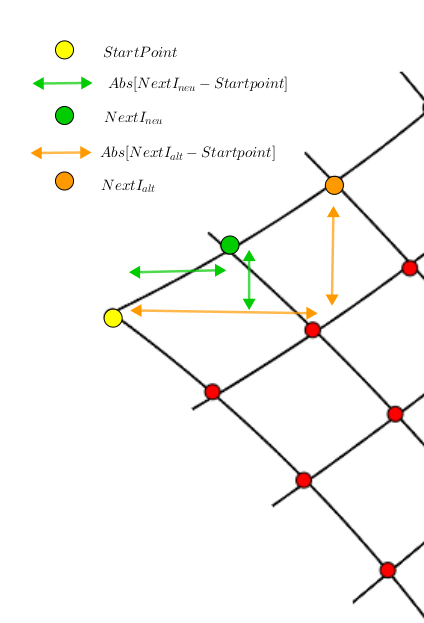
\includegraphics[width=0.5\linewidth]{images/SearchNextI.png}
	\caption[Überprüfung des gefundenen $NextI$]{Um zu überprüfen, ob der momentan $NextI$, in der Abbildung der orange Punkt, wirklich der nächste Punkt ist, wird sein Abstand zum Starpunkt in $j$- und  $i$- Richtung, mit den anderen noch möglichen Punkten verglichen. Gibt es einen dessen beide Abstände kleiner sind, wie beispielsweise der grüne Punkt, so wird dieser zum neuen $NextI$ bestimmt.}
	\label{fig:FindNextIJ}
\end{figure}


Mit den Punkten $StartPoint$, $NextI$ und $NextJ$ können die ersten Richtungsvektoren gebildet werden, anhand welcher das Schachbrett Gitter rekonstruiert werden kann. Für beide Richtungen wird die Anzahl der möglichen Punkte begrenzt. Es werden zwei Listen $IList$ und $JList$ angelegt. In $IList$ werden alle Punkte innerhalb der Zellen $CellI_{min}$ bis $CellI_{max}$ und $CellJ_1$ und $CellJ_2$ gespeichert. In Abbildung \ref{fig:IListJList} entspricht das dem Vertikalen blauen Bereich. In $JList$, kommen alle Punkte innerhalb von $CellJ_{min}$ bis $CellJ_{max}$ und $CellI_1$ und $CellI_2$. Was dem horizontalen blauen Bereich in Abbildung \ref{fig:IListJList} entspricht. \\

Zuerst wird die erste Kante in $j$-Richtung vervollständigt. Es wird ein Richtungsvektor $NextJDir$ aus $StartPoint$ und $NextJ$ gebildet. Des Weiteren wird ein Pufferwert $ProportionI$ deklariert, welcher den $i$-Koordinatenabstand zwischen $StartPoint$ und $NextJ$ beinhaltet. Anhand des Richtungsvektors $NextJDir$ und des Pufferwertes $ProportionI$ wird der nächste Punkt von $NextJ$ aus gesucht. \\

\begin{gather*}
	NextJDir = NextI - StartPoint\\
	ProportionI = NextI[CoordI]-StartPoint[CoordI]
\end{gather*}\\

In Abbildung \ref{fig:IListJList} auf dem linken Bild wird der Richtungsvektor $NextJDir$ als Pfeil vom gelben $StartPoint$ zum roten $NextJ$ dargestellt, der Richtungsvektor wird noch um einen Pufferwert vergrößert, da durch Perspektive und Bildverzerrungen die Abstände zwischen den einzelnen Punkten nicht mehr einheitlich sein muss. Die Pfeile welche in $i$-Richtung von $NextJ$ aus ausgehen, ist der Abstand $ProporionI$, welcher auf die $i$-Koordinate von $NectJ$ einmal addiert und einmal subtrahiert wird. Der Bereich den die Vektoren aufspannen bildet den Suchbereich für den auf $NextJ$ folgenden Punkt.\\

%\begin{figure}[!htb]
%	\minipage{0.48\textwidth}
%	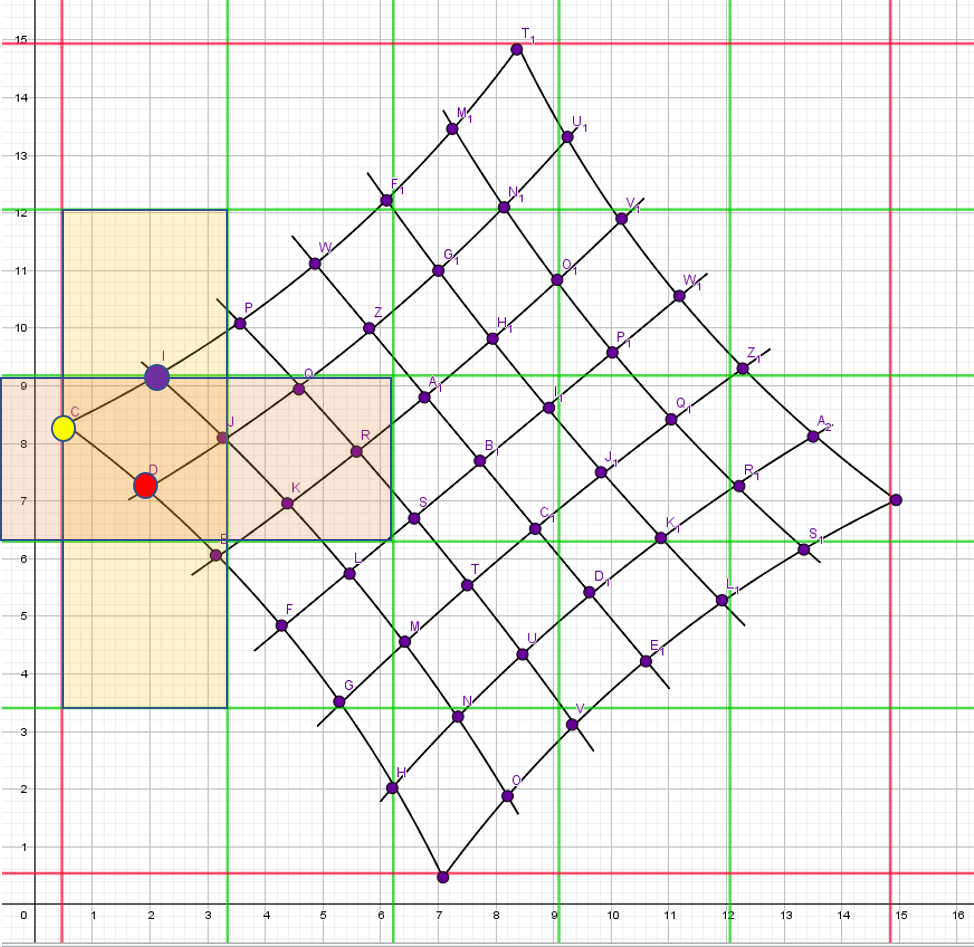
\includegraphics[width=\linewidth]{images/VerzeichnetesSchachbrett_2.png}
%	\caption{}
%	\label{fig:awesome_image1}
%	\endminipage\hfill
%	\minipage{0.48\textwidth}
%	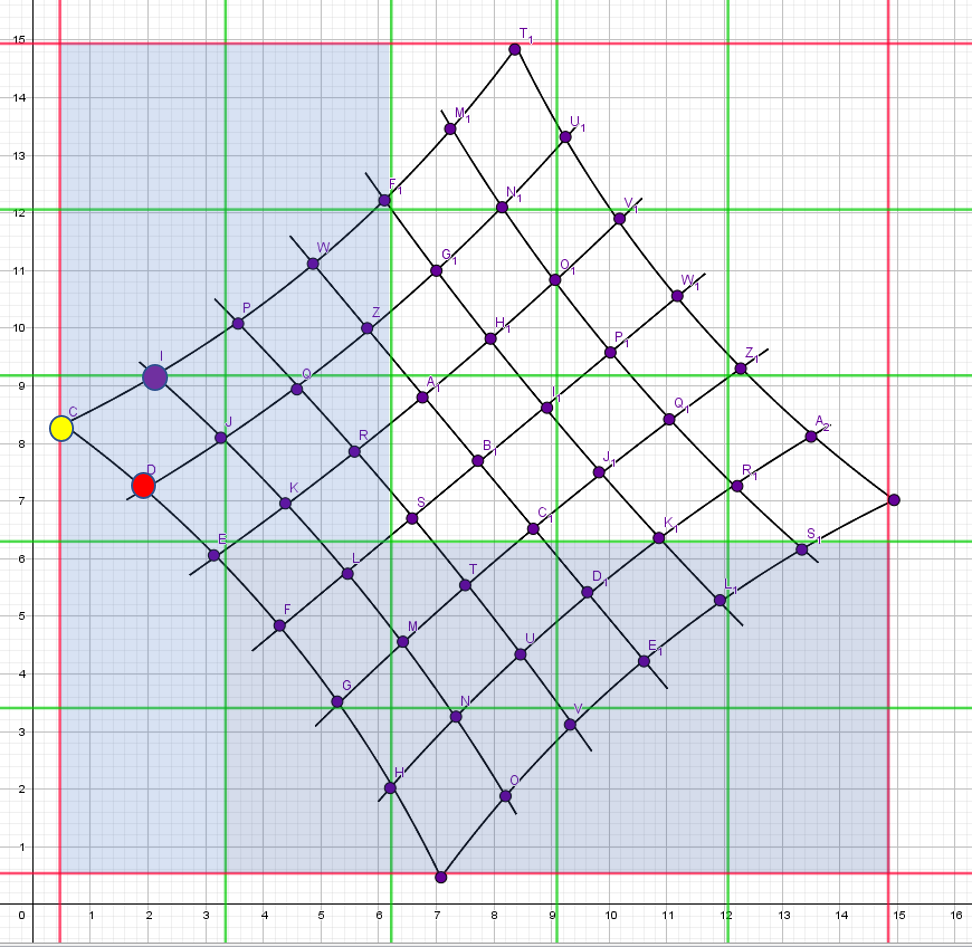
\includegraphics[width=\linewidth]{images/VerzeichnetesSchachbrett_3.png}
%	\caption{}
%	\label{fig:awesome_image2}
%	\endminipage\hfill
%	%	\caption{Die mit dem \textit{SURF}-Algorithmus gefundenen Punkte sind mit den gelben Ziffern im Bild gekennzeichnet}
%\end{figure}

\begin{figure}[!htb]
	\centering
	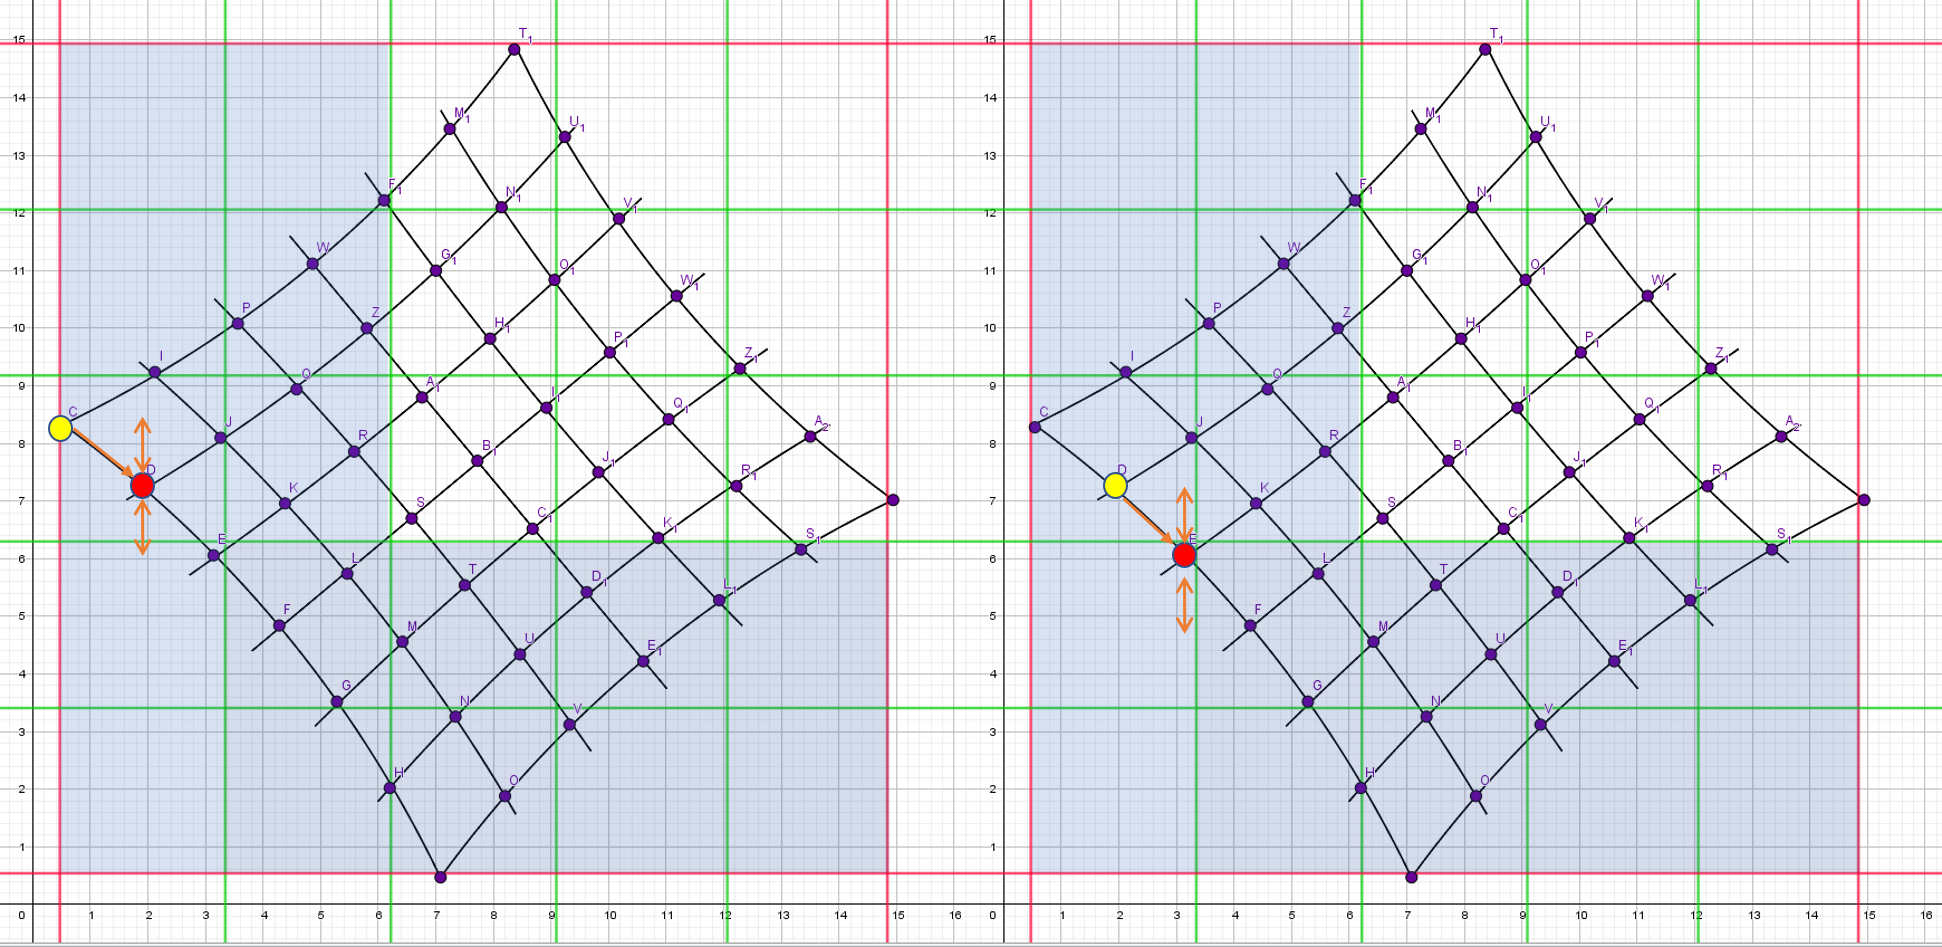
\includegraphics[width=1\linewidth]{images/VerzeichnetesSchachbrett_4.png}
	\caption[Suche nach $NextJ$]{Im linken Bild ist der Startpunkt in gelb dargestellt und der bereits gefundenen Punt $NextJ$ ist in rot eingefärbt. Anhand der beiden Punkte wird ein Richtungsvektor definiert und zwei Pufferwerte oberhalb und unterhalb. Diese bilden einen Suchbereich. Im rechten Bild wurde $NextJ$ als neuer Startwert festgelegt. Der zuvor definierte Suchbereich wird vor den neuen Startpunkt gesetzt und es wird nach einem potentiellen nächsten $NextJ$ gesucht.}
	\label{fig:IListJList}
\end{figure}

$NextJ$ wird zum neuen $StartPoint$. Vom neuen $StartPoint$ ausgehend, wird der zuvor definierte Suchbereich nach einem neuem $NextJ$ abgesucht. Wird ein Punkt in diesem Bereich entdeckt, so wird dieser zum neuen $NextJ$, sofern er sich noch nicht in der $CheckList$ befindet. Tritt der Fall ein, dass ein Punkt bereits in der $CheckList$ sich befindet, so wird dieser ignoriert. Die Position und der Platz im Schachbrettgitter werden dem neu entdeckten Punkt, wie die Punkten zuvor, durch Schlüsselwerte festgehalten und in die Liste $SortedList$ gespeichert. Des Weiteren wird auch dieser in die $CheckList$ aufgenommen.\\

Anhand des neuen $StartPoints$ und des neuen $NextJ$ werden der Richtungsvektor $NextJDir$ und $ProportionI$ neu berechnet. $NextJ$ wird wieder zum neuen $StartPoint$ und die Suche wird dementsprechend weiter geführt, bis kein Punkt mehr gefunden wird. Alle Punkte werden als $Asssociation$ mit entpsrechenden Schlüsselwerten in $SortedList$ und $CheckList$ eingetragen.\\

Bevor die Suche jedoch beendet wird, treten noch zwei Sicherheitsfunktionen in Kraft. Die erste wird als $Saftylist$ bezeichnet. Wird beispielsweise kein weiterer Punkt innerhalb von $JList$ gefunden, so erweitert $Saftylist$ den Suchbereich um den letzten noch detektierten $NextJ$ um alle Zellen um diesen Punkt herum und überprüft, dann nochmal, ob es einen weiteren Punkt innerhalb des letzten definierten Suchbereiches gibt. Ist dies der Fall, so wird dieser Punkt auch noch mit aufgenommen. Ist dies nicht der Fall ist die Suche für die Reihe beendet. Die selbe Sicherheitsfunktion gibt es auch für die Suche in $i$-Richtung.\\

In Abbildung \ref{fig:SaftyList} auf dem rechten Bild ist ein Beispiel für den Einsatz der $SaftyList$-Funktion zu sehen. Der rote Bereich vom gelben Punkt aus gehend ist definiert als der Bereich potentieller weiterer Punkte außerhalb der $IList$.\\

Ist die erste $j$-Kante bestimmt, so wird die nächste Reihe vervollständigt, beginnend am Punkt $NextI$. Danach muss in $i$-Richtung zunächst der nächste $NextI$ bestimmt werden, damit aufbauend auf diesem die nächste Reihe in $j$-Richtung vervollständigt werden kann. Wie in den Abbildung \ref{fig:FindNextIPoint} und \ref{fig:SaftyList} zu sehen, basiert die Suche nach $NextI$ auf dem gleichen Verfahren wie die Suche nach $NextJ$.\\


\begin{figure}[!htb]
	\centering
	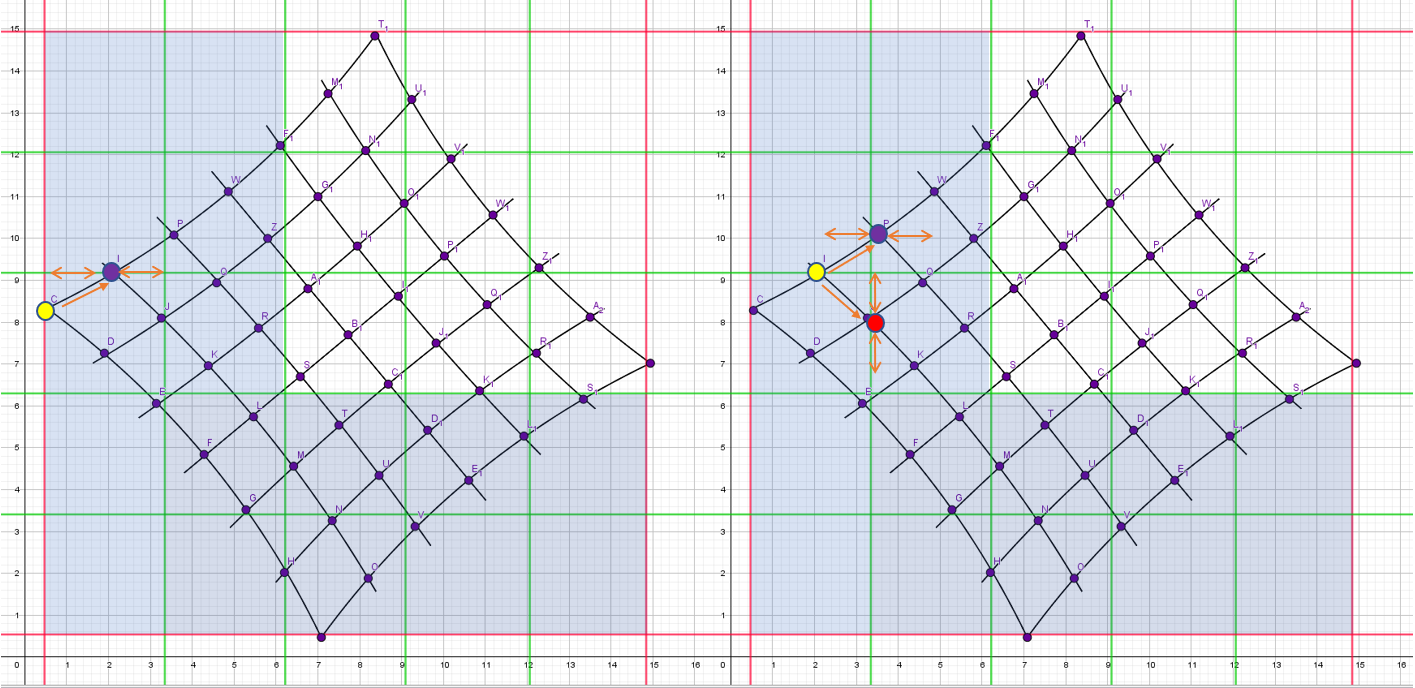
\includegraphics[width=1\linewidth]{images/VerzeichnetesSchachbrett_5.png}
	\caption[Suche nach dem nächsten $NextI$]{Die Suche nach dem nächsten $NextI$ basiert auf dem selben Verfahren wie die Suche nach $NextJ$. Sobald ein neuer $NextI$ gefunden wurde, wird die Reihe in $j$-Richtung vervollständigt, bevor es mit dem nächsten $NextI$ weiter geht}
	\label{fig:FindNextIPoint}
\end{figure}

\begin{figure}[!htb]
	\centering
	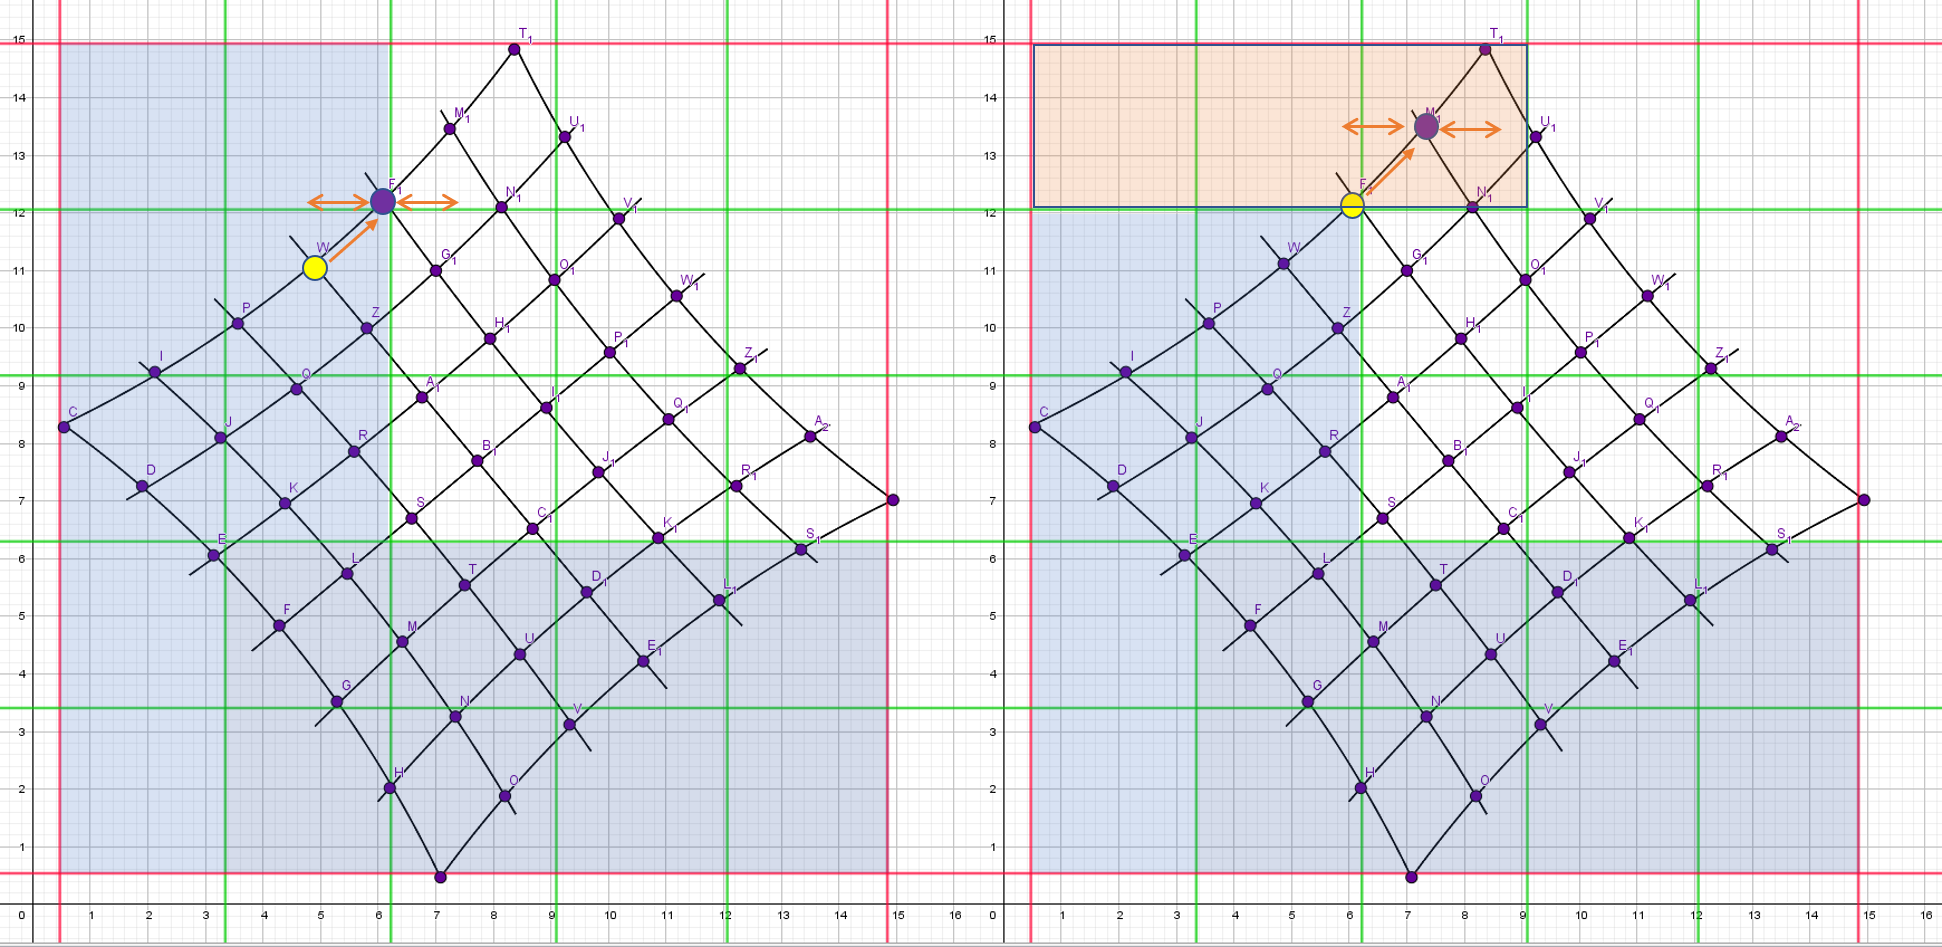
\includegraphics[width=1\linewidth]{images/VerzeichnetesSchachbrett_6.png}
	\caption[Sicherheitsfunktion $SaftyList$]{Wird der kein weiterer Punkt innerhalb von $IList$ oder $JList$ gefunden, Wird ein kleiner Bereich, hier in rot hinterlegt, abgesucht, ob es doch noch potentielle nächste Punkte gibt, die aufgrund der Lage des Schachbretts nich in $IList$ oder $JList$ mit enthalten waren}
	\label{fig:SaftyList}
\end{figure}

Zuvor wurde erwähnt, dass es neben $SaftyList$ noch eine andere Funktion, welche die Detektion aller Punkte absichert. Hierzu sei nochmal erwähnt, dass der hier beschriebene Sortierungsalgorithmus auf einem bereits bestehenden Algorithmus aufbaut. Dieser Algorithmus detektiert Die Eckpunkte eines Schachbretts. Bei der Detetktion kann es vorkommen, dass Punkte nicht erkannt werden. Ist dies der Fall entstehen Lücken im Schachbrettmuster und der Sortierungsalgorithmus, würde nicht alle Punkte richtig sortieren könne.\\

Um das zu verhindern, wurde eine Sicherheitsfunktion eingebaut. Sollte es vorerst kein Punkt im Suchbereich entdeckt, werden, so setzt die Sicherheitsfunktion einen synthetischen Punkt und sucht ausgehend von diesem synthetischen weiter nach Punkten. Sollte ein Punkt nach dem synthetischen Punkt gefunden werden, so bleibt der synthetische Punkt bestehen und die Suche wird normal fortgesetzt. Wird nach dem setzten des synthetischen Punkt kein weiterer Punkt gefunden, gilt die Suche in der Reihe beziehungsweise Spalte für beendet.\\

In Abbildung \ref{fig:ChessBoardLeft} und \ref{fig:ChessBoardRight} wird ein Schachbrett aus zwei unterschiedlichen Blickwinkeln dargestellt. Die roten Punkte markieren die Eckpunkte, deren Koordinaten an den Sortierungsalgorithmus übergeben werden. In den Abbildungen \ref{fig:ChessBoardLeftAlg} und \ref{fig:ChessBoardRightAlg} werden alle Punkte, welche in der Liste $SortedPoints$ gespeichert wurden in einem Plot ausgegeben. Es wird gesagt, dass alle Punkte deren Schlüssel $NeighbourI = 3$ ist, in grün dargestellt werden sollen. Das Ergebnis dieser Abfrage ist ebenfalls in den Abbildungen \ref{fig:ChessBoardLeftAlg} und \ref{fig:ChessBoardRightAlg} zu sehen. Der entstandene Sortierungalgorithmus ist also in der Lage aus Bildern zweier Schachbretter gleiche Eckpunkte und somit korrespondierende Punkte zu detektieren. 


\begin{figure}[!htb]
	\minipage{0.47\textwidth}
	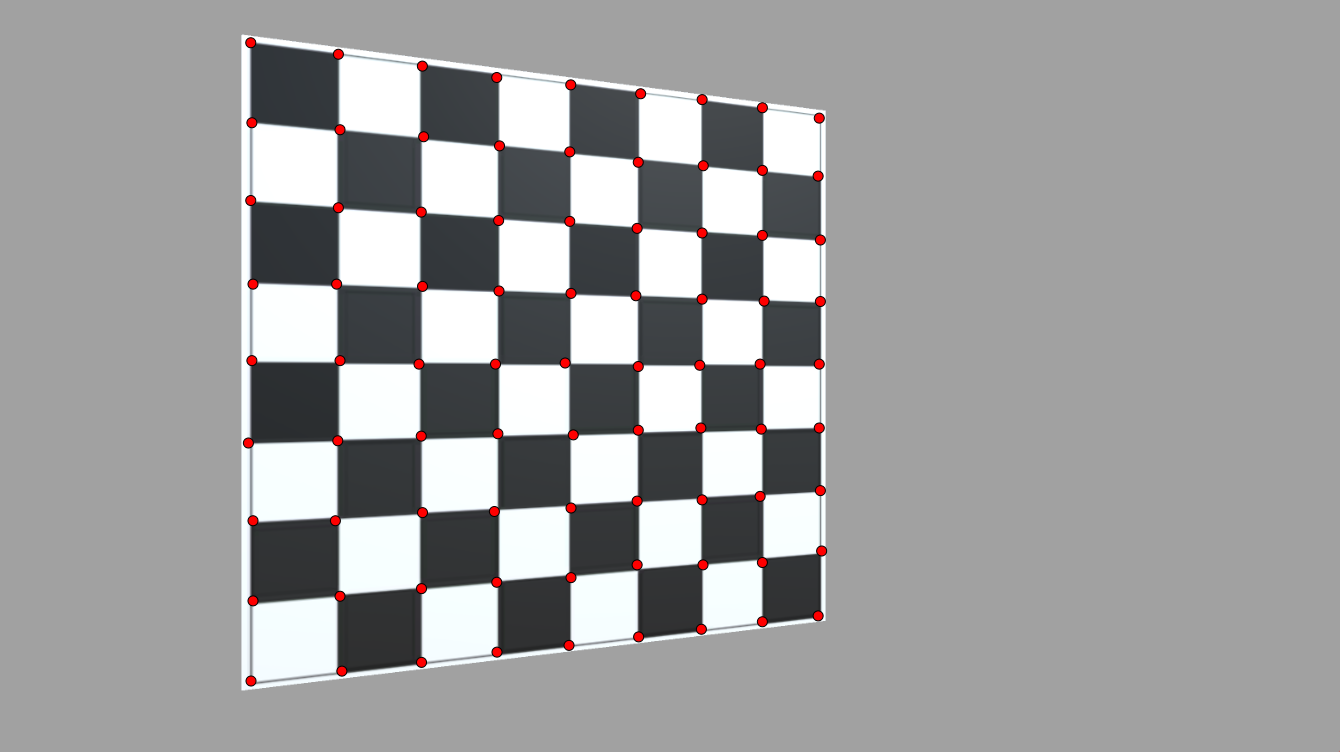
\includegraphics[width=\linewidth]{images/ChessBoardLeft.png}
	\caption[Korrespondezsuche mit Sortierungsalgorithmus. Schachbrett auf linker Seite]{Die Kamera,welche das Schachbrett abbildet steht links versetzt zum Schachbrett und ist rotiert}
	\label{fig:ChessBoardLeft}
	\endminipage\hfill
	\minipage{0.48\textwidth}
	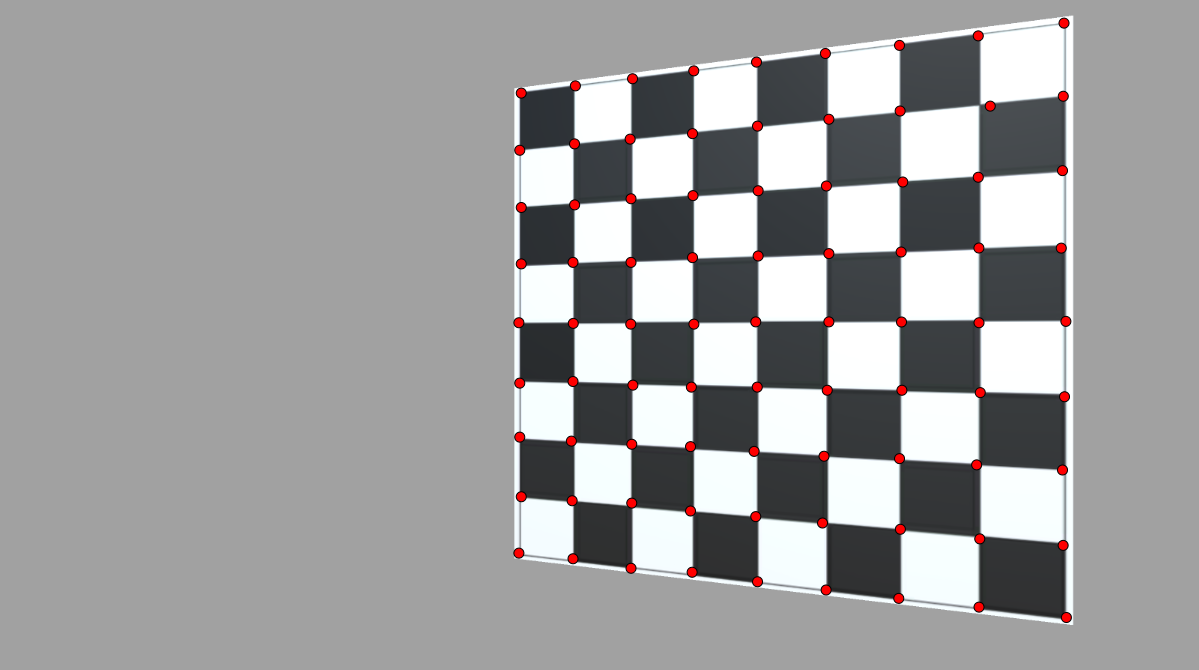
\includegraphics[width=\linewidth]{images/ChessBoardRight.png}
	\caption[Korrespondezsuche mit Sortierungsalgorithmus. Schachbrett auf rechter Seite]{Die Kamera, welche das Schachbrett abbildet steht rechts versetzt zum Schachbrett und ist rotiert}
	\label{fig:ChessBoardRight}
	\endminipage\hfill
\end{figure}


\begin{figure}[!htb]
	\minipage{0.48\textwidth}
	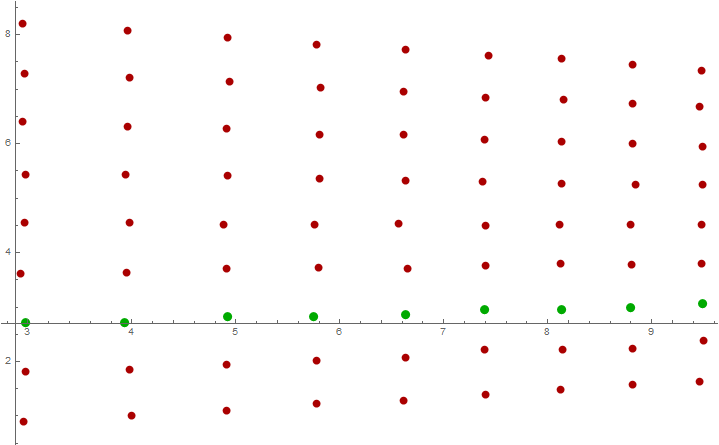
\includegraphics[width=\linewidth]{images/ChessBoardLeftAlg.png}
	\caption[Ergebnis des Sortierungsalgorithmus. Schachbrett auf linker Seite]{Die Abbidlung zeigt das Ergebnis der Sortierung des linken Schachbretts. In grün ist die Reihe an Punkten zu sehen, welche den Schlüssel $NeighbourI = 3$ haben.}
	\label{fig:ChessBoardLeftAlg}
	\endminipage\hfill
	\minipage{0.48\textwidth}
	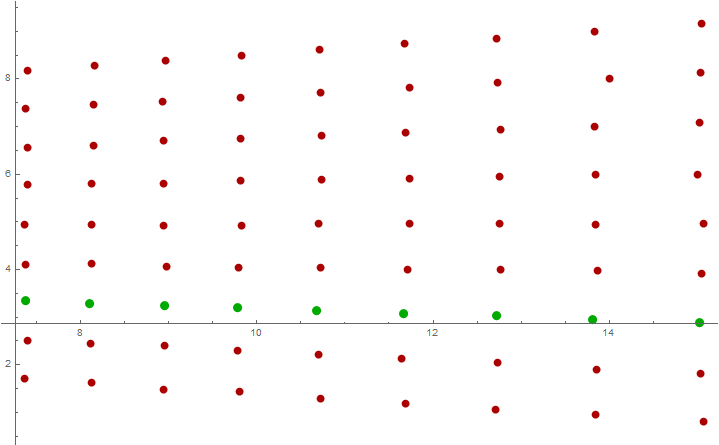
\includegraphics[width=\linewidth]{images/ChessBoardRightAlg.png}
	\caption[Ergebnis des Sortierungsalgorithmus. Schachbrett auf linker Seite]{Die Abbidlung zeigt das Ergebnis der Sortierung des rechten Schachbretts. In grün ist die Reihe an Punkten zu sehen, welche den Schlüssel $NeighbourI = 3$ haben.}
	\label{fig:ChessBoardRightAlg}
	\endminipage\hfill
\end{figure}
\pagebreak


\section{Resultate bei stark verzerrten Schachbrettern}
\label{sec:SchachAlgBeispiele}

Der entstandenen Sortierungsalgorithmus wird an stark perspektivisch Verzerrten oder durch Bildfehler wie Verzeichnungen betroffenen Schachbrettern getestet. Auch hier wird gesagt, dass sich die Punkte deren Schlüssel $NeighbourI = 3$ ist grün einfärben sollen. Die Abbildungen \ref{fig:Extreme1} bis \ref{fig:Extreme10} zeigen die Resultate der Punktesortierung in start verzerrten Schachbrettgittern.


%In den folgenden Beispielen sieht man jeweils das Originalbild und ein Bild welches die durch den Algorithmus sortierten Punkte farbig ausgibt. Die grünen eingefärbten Punkte sind in den Bildern des Algorithmus die Nachbarn, welche sich in i-Richtung an der dritten Stelle befinden. Natürlich können auch andere Reihen oder auch einzelne Punkte abgefragt werden. 


\begin{figure}[!htb]
	\minipage{0.48\textwidth}
	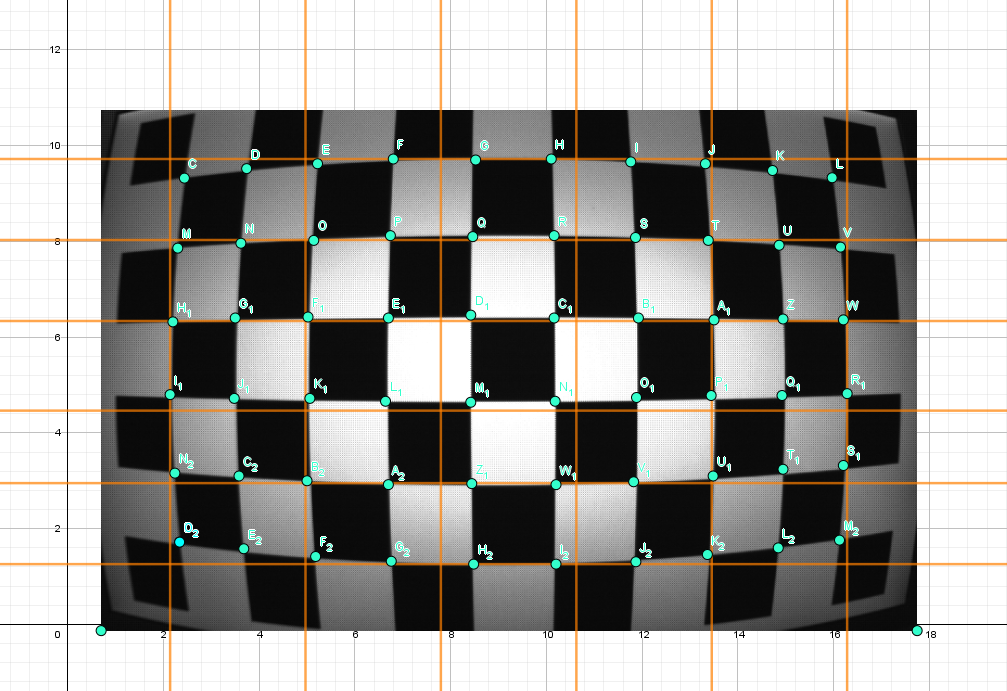
\includegraphics[width=\linewidth]{images/Tonnenverzeichnung.png}
	\caption[Schachbrett mit Tonnenverzeichnung]{Schachbrett mit Tonnenverzeichnung}
	\label{fig:Extreme1}
	\endminipage\hfill
	\minipage{0.48\textwidth}
	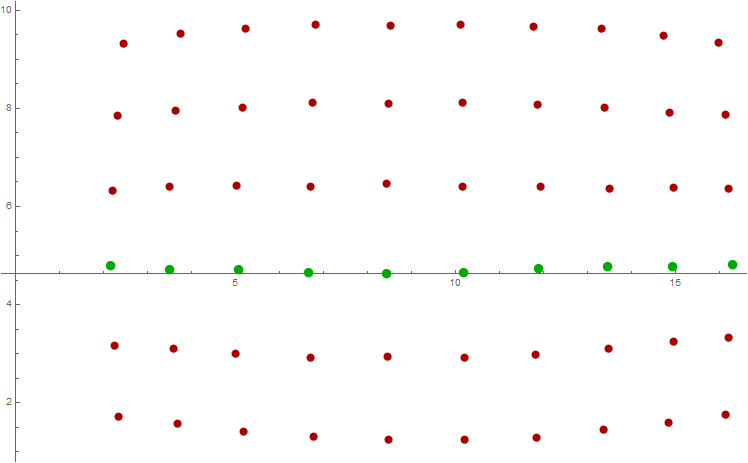
\includegraphics[width=\linewidth]{images/AlgTonnenverzeichnung.png}
	\caption[Sortierte Punkte eines Schachbretts mit Tonnenverzeichnung]{Ergebnis des Sortierungsalgorithmus.}
	\label{fig:Extreme2}
	\endminipage\hfill
\end{figure}

\begin{figure}[!htb]
	\minipage{0.45\textwidth}
	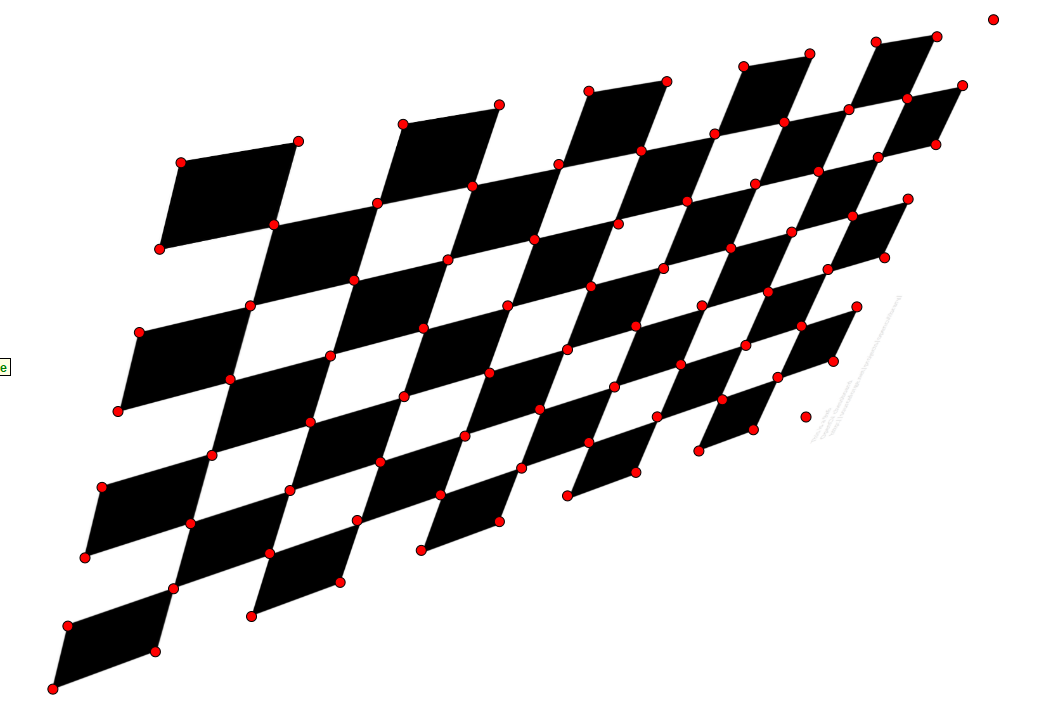
\includegraphics[width=\linewidth]{images/perspektivisch.png}
	\caption[perspektivisch startk verzerrtes Schachbrett]{Perspektivisch stark verzerrtes Schachbrett}
	\label{fig:Extreme3}
	\endminipage\hfill
	\minipage{0.49\textwidth}
	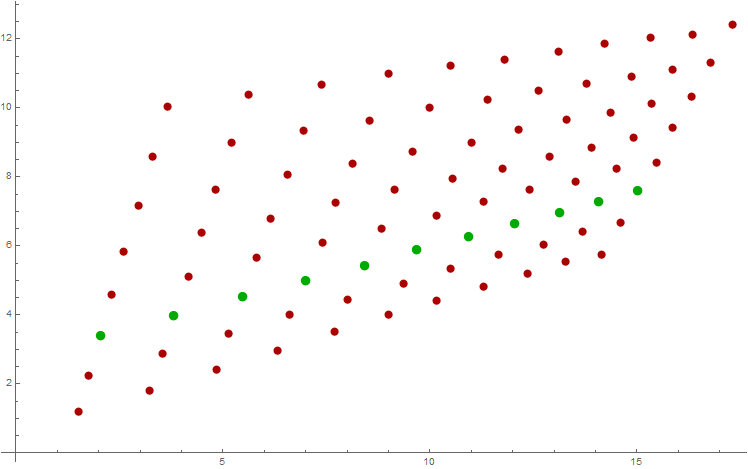
\includegraphics[width=\linewidth]{images/AlgPerspektifisch.png}
	\caption[Sortierte Punkte eines perspektivisch verzerrten Schachbretts]{Ergebnis des Sortierungsalgorithmus.}
	\label{fig:Extreme4}
	\endminipage\hfill
\end{figure}


\begin{figure}[!htb]
	\minipage{0.48\textwidth}
	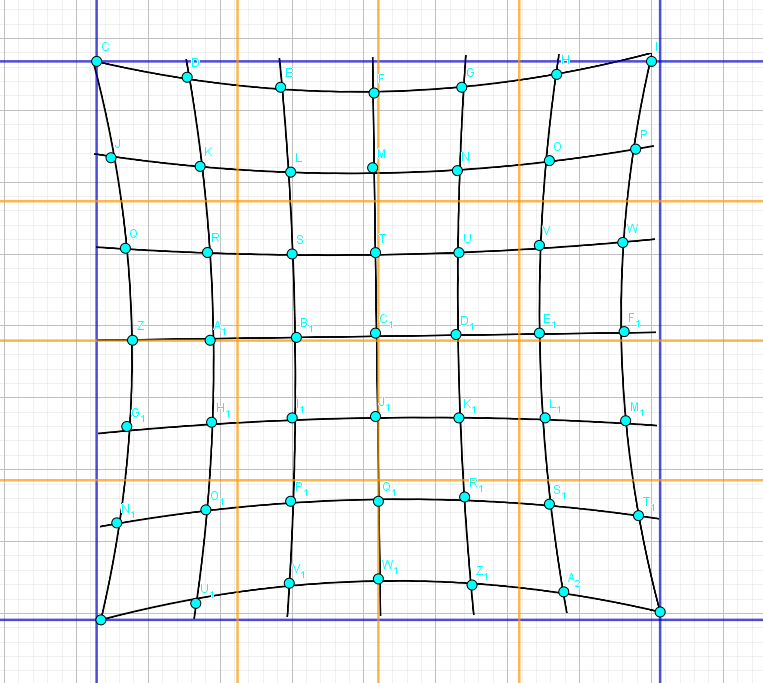
\includegraphics[width=\linewidth]{images/KissenVerzeichnung.png}
	\caption[Schachbrett mit Kissenverzeichnung]{Schachbrett mit Kissenverzeichnung}
	\label{fig:Extreme5}
	\endminipage\hfill
	\minipage{0.50\textwidth}
	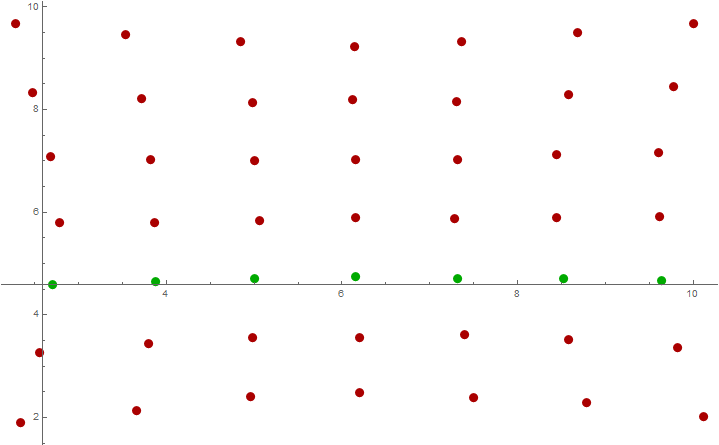
\includegraphics[width=\linewidth]{images/AlgKissen.png}
	\caption[Sortierte Punkte eines Schachbretts mit Kissenverzeichnung ]{Ergebnis des Sortierungsalgorithmus.}
	\label{fig:Extreme6}
	\endminipage\hfill
\end{figure}

\begin{figure}[!htb]
	\minipage{0.48\textwidth}
	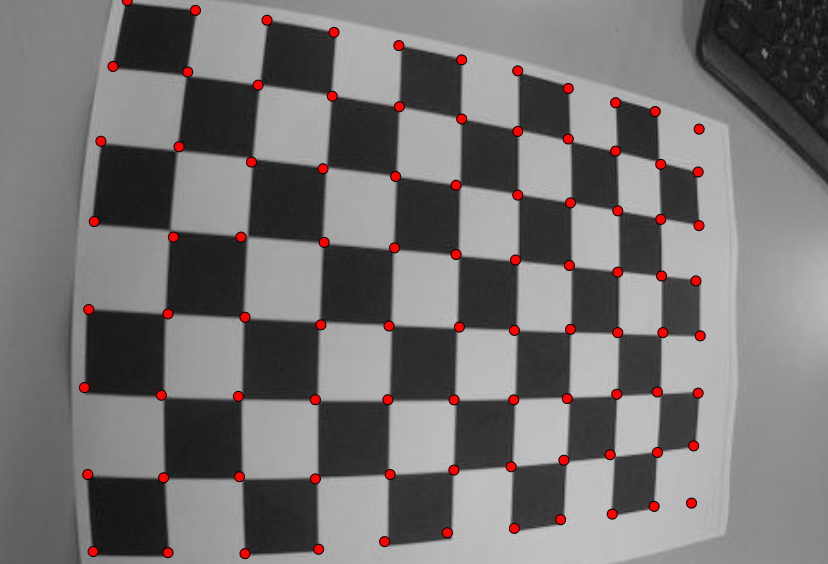
\includegraphics[width=\linewidth]{images/Tonnenverzeichnung_Perspektivisch.png}
	\caption[Perspektivisch verzerrtes Schachbrett mit Tonnenverzeichnung]{Perspektivisch verzerrten Schachbrett mit Tonnenverzeichnung}
	\label{fig:Extreme7}
	\endminipage\hfill
	\minipage{0.48\textwidth}
	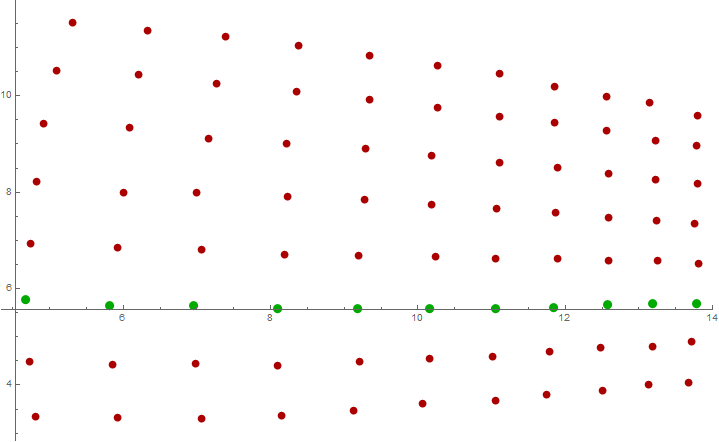
\includegraphics[width=\linewidth]{images/Tonnenverzeichnung_Perspektivisch_Alg.png}
	\caption[Sortieret Punkte eines perspektivisch verzerrten Schachbretts mit Tonnenverzeichnung]{Ergebnis des Sortierungsalgorithmus.}
	\label{fig:Extreme8}
	\endminipage\hfill
\end{figure}

\begin{figure}[!htb]
	\minipage{0.48\textwidth}
	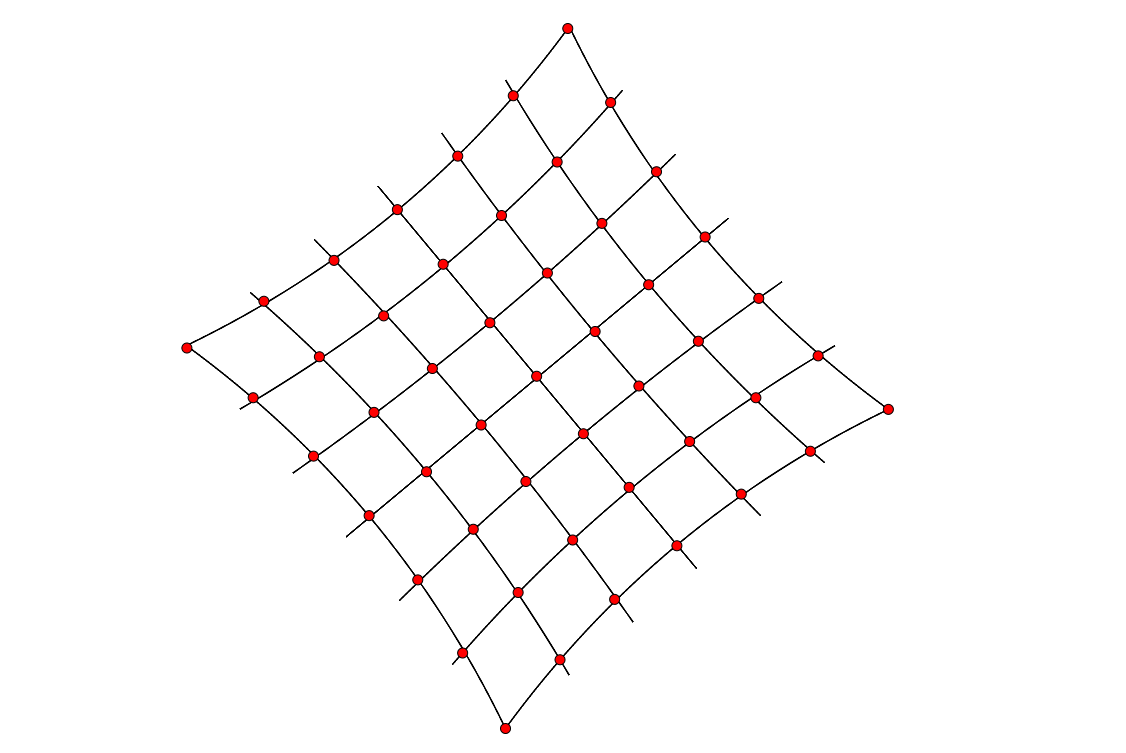
\includegraphics[width=\linewidth]{images/extrBsp.png}
	\caption{Bild eines Tonnenförmig verzeichnetem leicht perspektivisch verzerrtem Schachbretts}
	\label{fig:Extreme9}
	\endminipage\hfill
	\minipage{0.48\textwidth}
	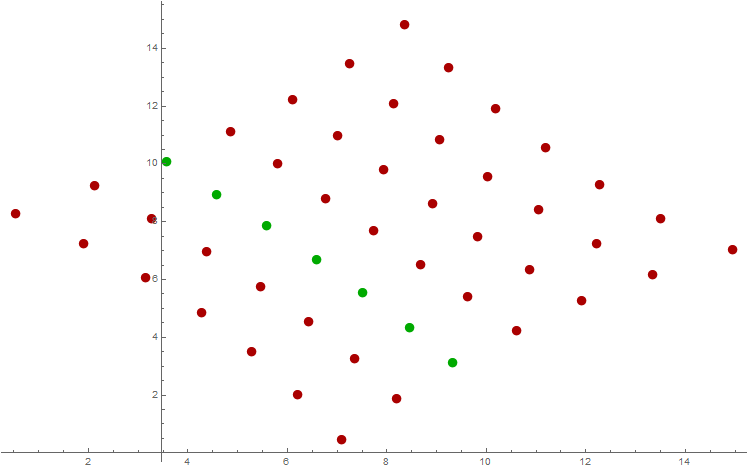
\includegraphics[width=\linewidth]{images/AlgExtrBsp.png}
	\caption{Algorithmisch detektierte Linie der dritten i-Reihe}
	\label{fig:Extreme10}
	\endminipage\hfill
\end{figure}


%\section{Modulübersicht}
%
%
%\begin{minipage}{\linewidth}
%	\centering
%	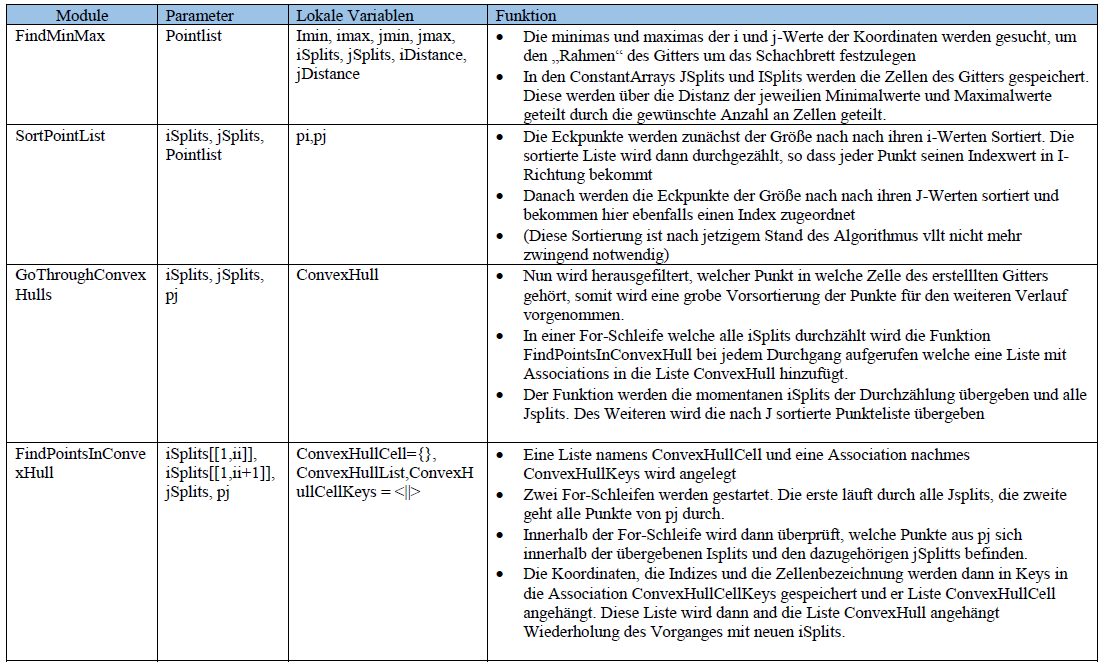
\includegraphics[width=1\linewidth]{images/KD1.png}
%	\captionof{figure}{Klassendiagramm}
%\end{minipage}
%\begin{minipage}{\linewidth}
%	\centering
%	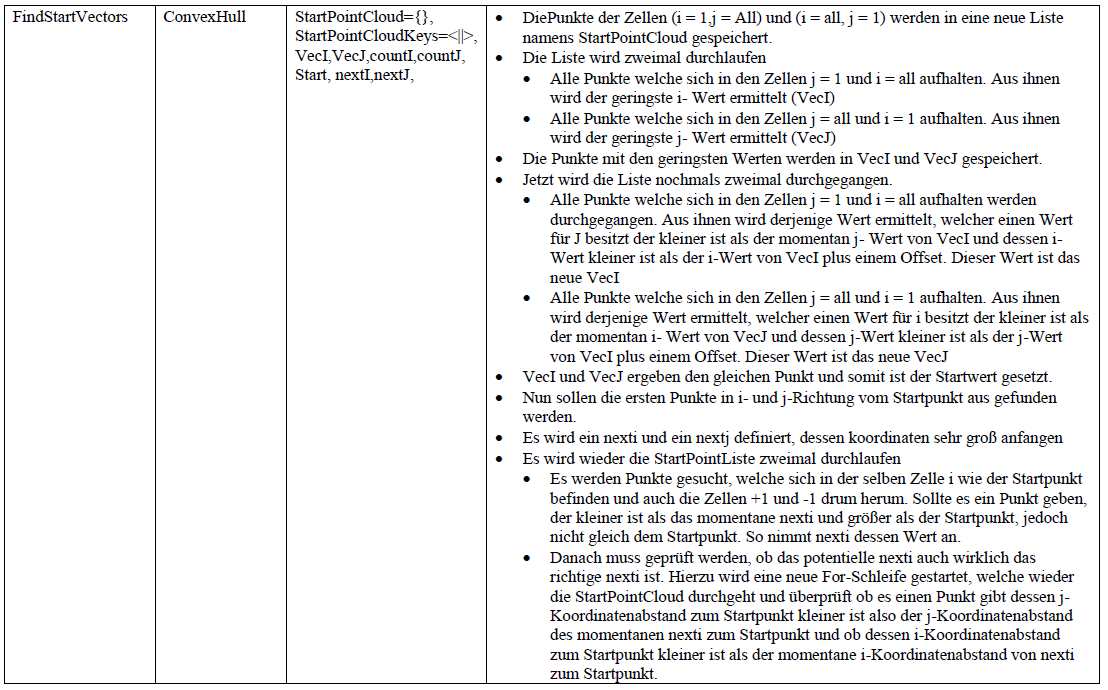
\includegraphics[width=1\linewidth]{images/KD2.png}
%	\captionof{figure}{Klassendiagramm}
%\end{minipage}
%\begin{minipage}{\linewidth}
%	\centering
%	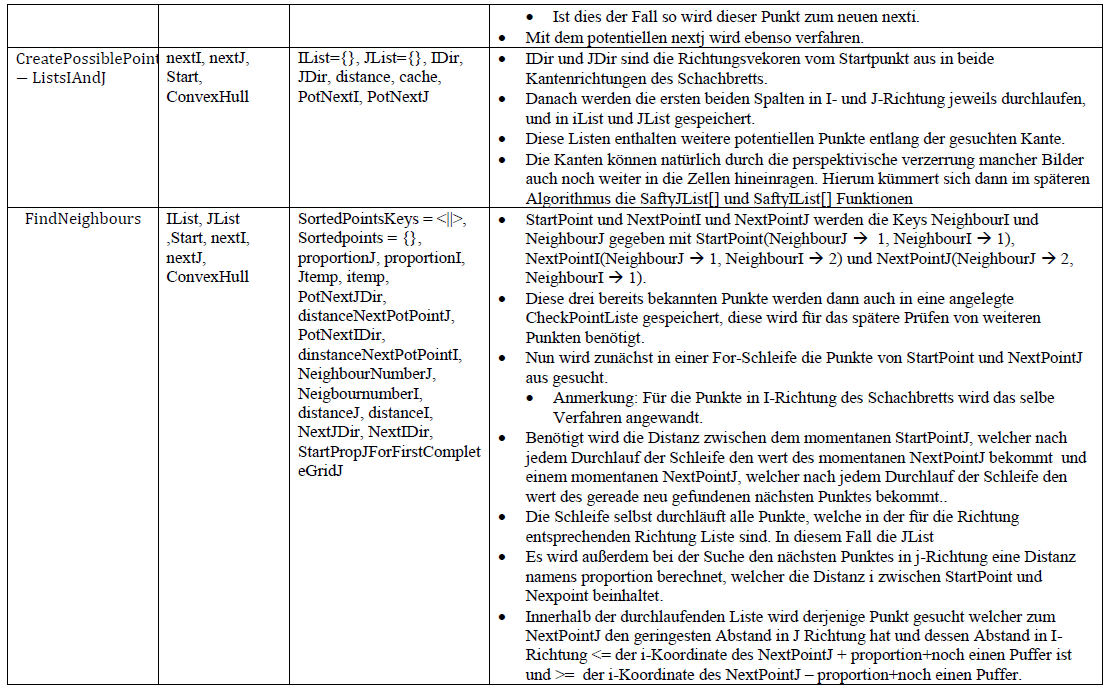
\includegraphics[width=1\linewidth]{images/KD3.png}
%	\captionof{figure}{Klassendiagramm}
%\end{minipage}
%\begin{minipage}{\linewidth}
%	\centering
%	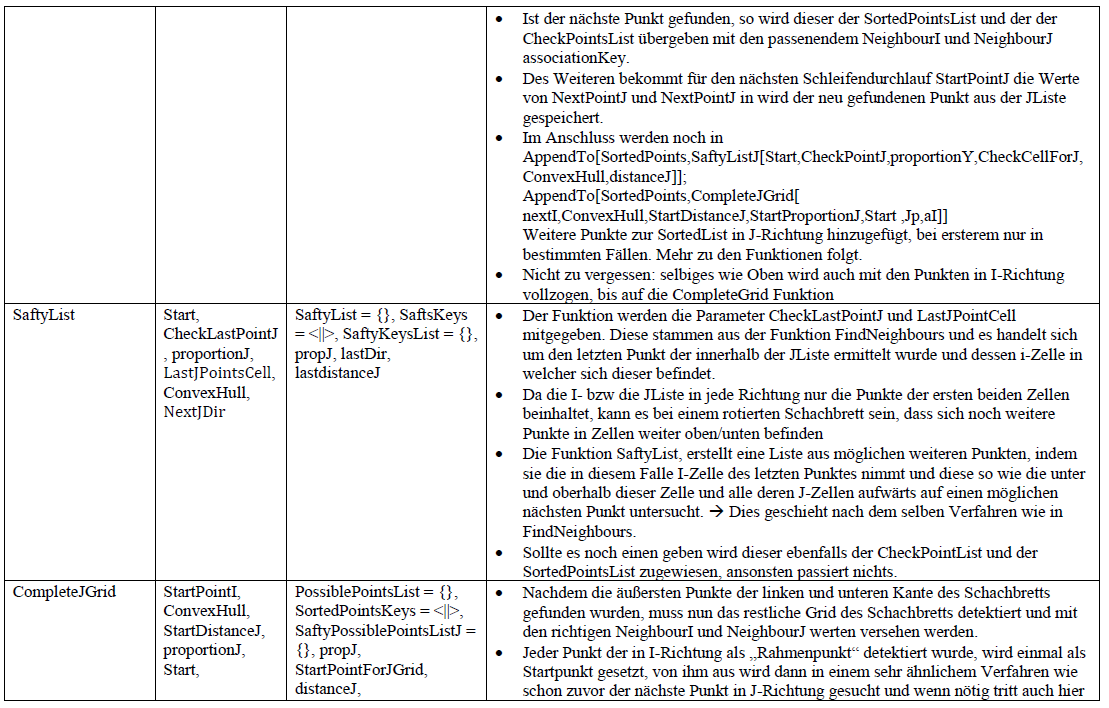
\includegraphics[width=1\linewidth]{images/KD4.png}
%	\captionof{figure}{Klassendiagramm}
%\end{minipage}
%\begin{minipage}{\linewidth}
%	\centering
%	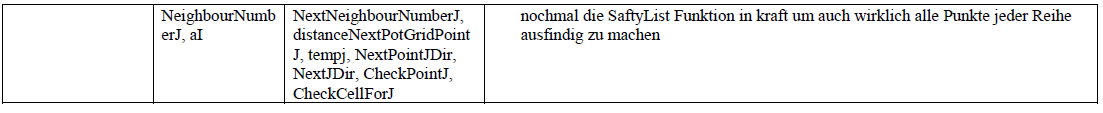
\includegraphics[width=1\linewidth]{images/KD5.png}
%	\captionof{figure}{Klassendiagramm}
%\end{minipage}\\


%Modulübersicht vllt in den Anhang??






